  \begin{titlepage}
    \begin{center}
    {\large \textsc{notes to}}
    \vskip 3ex

    {\Huge Feeling Gravity's Pull}
    \vskip 4.2ex

    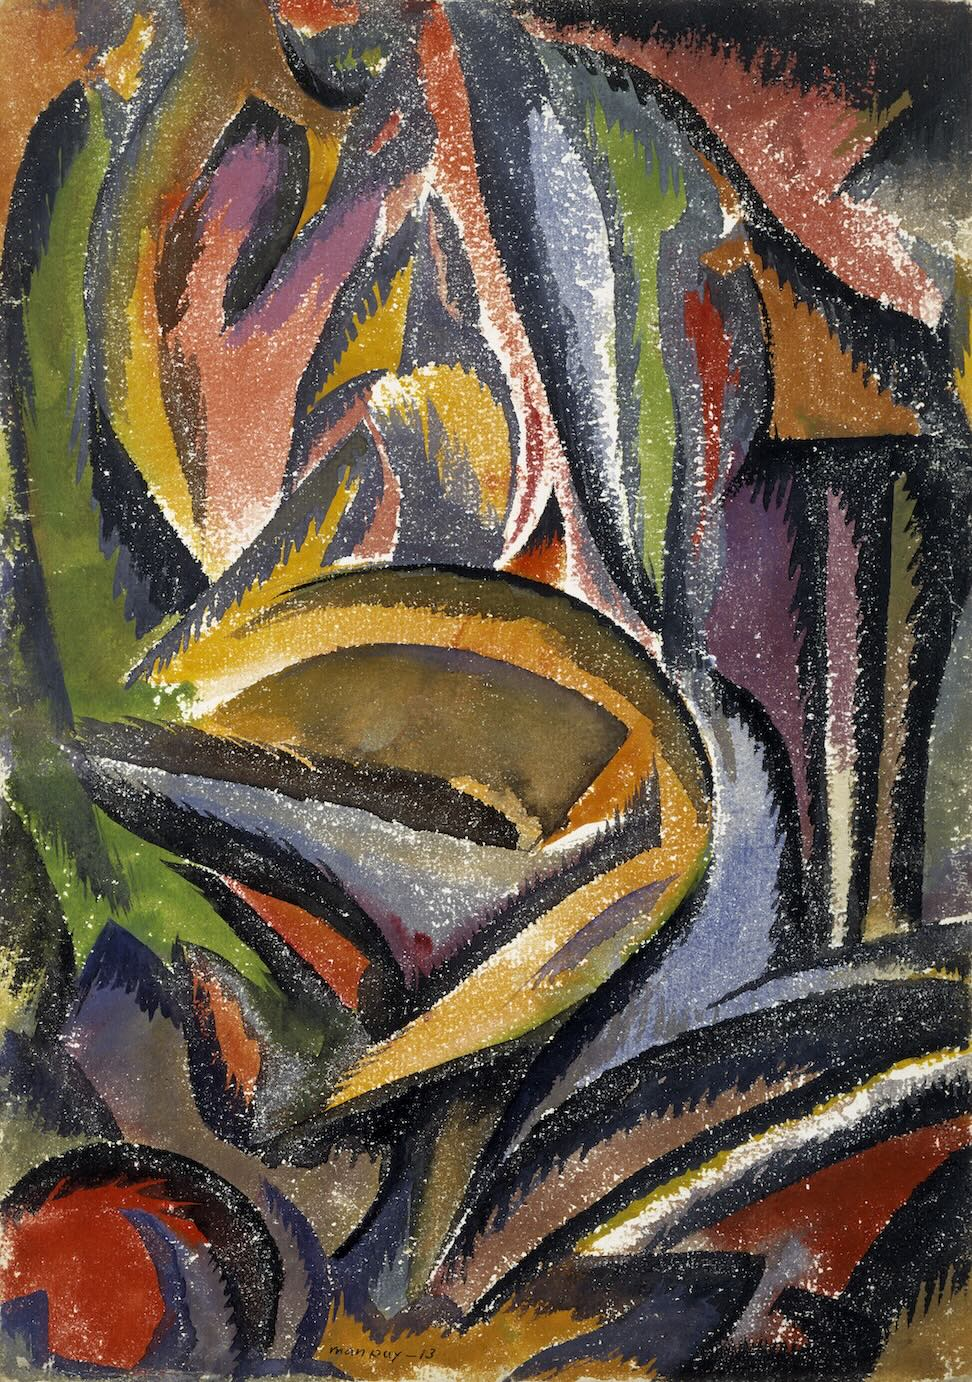
\includegraphics{lib/Man_Ray_Kinda_Sky_compressed}
    \end{center}
    {\small Man Ray, \textit{Landscape (Paysage Fauve)} (watercolor, 1913), \textit{in} \textsc{Smithsonian Museum Am.~Art}, \url{https://americanart.si.edu/artwork/landscape-paysage-fauve-31825} (last visited Jan. 23, 2024).}\footnote{I'm not sure if this is what R.E.M. means when they say ``A Man Ray kind of sky,'' but it's what I always think of. \textsc{R.E.M.}, \textit{Feeling Gravity's Pull, on} \textsc{Fables of the Reconstruction} (I.R.S. Records, 1985).}

    \vskip 4.2ex
    \centering
    {\large \textsc{V{\ae}gtersang}}

    Last Revised: \today
  \end{titlepage}
  \newpage
  \addcontentsline{toc}{section}{Contents}
  \tableofcontents
  \newpage
